\subsection{Preprocessing}
%In this sub-section,we describe the preprocessing step
%on Wikipedia corpus.
%\KZ{Why both wiki and plain text, don't we only iterate on wiki docs here?}
We start from the generation
of the term-sense mapping from Wikipedia corpus.
Then we introduce our parsing method on
Wikipedia articles by making use of an NLP chunker.

\subsubsection{Generate Term-Sense Mapping}
%\KZ{Why do we need the candidate sense list?}
To identify the sense of an unlinked term, we need to know the candidate
senses of that term.
Each term may map to more than
one Wikipedia concepts which are the {\em senses}.
%In the following discussion, we will use the term {\em senses}
%and {\em concepts} interchangeably.
The list of all Wikipedia concepts associated with an unlinked term is called
the candidate sense list.
In this paper, we use three sources in Wikipedia to build the
term-sense mapping:
Wikipedia article titles, redirect pages and disambiguation pages.
Specifically, each Wikipedia concept (sense) is mapped to
%We collect the surface form of a Wikipedia concept/sense from
the title of this concept's article,
titles of redirect pages linked to this concept,
and the title of disambiguation pages that contain this concept.
%This collection forms term-sense mapping.
In other works such as Cucerzan's\cite{cucerzan2007large},
anchor text of links in Wikipedia articles are also used as
a source of mapping.
Our observation is that surface forms in the anchor text and the links
between the surface form and the Wikipedia article can both be
noisy and unreliable. Anchor texts are not necessarily MWEs
and the linked articles are sometimes not really the description of
the anchor text but are rather just ``related'' information.

%\myskip
\begin{example}
\label{ex:wronglink}
A further 6-7 million were {\uline{deported and exiled}}
 [linkto: {\em Population transfer in the Soviet Union}] to remote areas of
the USSR, and 4-5 million passed through ``labour colonies''.
\end{example}
%\myskip

\exref{ex:wronglink} shows a sentence from a Wikipedia article
named ``Gulag'' \cite{gulag}.
The anchor text ``deported and exiled'' is not a term, and the
concept  ``Population transfer in the Soviet Union'' is not exactly
a sense of ``deported and exiled.''
Due to this observation, we do not include links as a source for
generating the term-sense mapping.
Our candidate sense list for ``polar bear'' is, for example,
{\em Polar bear}, {\em Polar Bear (American band)}, {\em Snow Patrol},
{\em Polar Bear Pass}, etc.
%The candidate sense list will be used in later
%functions like parsing plain texts and updating co-occurrence matrix.


\subsubsection{Parse Text into Noun Phrases}
\label{sec:parse}
%In this sub-section, we describe the process of parsing texts into noun phrases.
%First, we prepare a {\em term list} which is comprised of all
%Wikipedia article titles, disambiguation page titles and redirect page titles.
With the term-sense mapping generated, we can now parse texts to
extract noun phrases.
First, we take all the surface forms in the term-sense mapping to
form a {\em term list}.
Only those noun phrases in the term list will be considered later.
%There are two scenarios for parsing. One is parsing plain texts with no
%links at all. This is used in the end-to-end wikification of a new document.
%The other scenario is parsing Wikipedia articles which contain some links.
%This is applicable in the iterative enrichment of current Wikipedia pages
%and the co-occurrence information.
In a Wikipedia article, we call terms which are already linked {\em linked terms},
while noun phrases which are waiting to be linked {\em unlinked terms}.
Next we introduce the details of parsing.
%in these two scenarios and then propose an optimization on both of
%the two scenarios so that the algorithm is more robust to parsing errors.

\begin{algorithm}[th]
\caption{Parsing a Chunk}
\label{parsechunk}
\begin{algorithmic}[1]
\Function{ParseChunk}{$Chunk$}
\State $Unlinked\leftarrow \emptyset$
\State $N\leftarrow wordCount(Chunk), k\leftarrow N$
\State $flag\leftarrow False$
\While {$k > 0\; and\; !flag$}
\State $candidateTerm \leftarrow Chunk[N-k,N]$
\If {$candidateTerm$ is $NP$}
\If {$candidateTerm \in TermList$}
\State Add $candidateTerm$ to $Unlinked$
\State $L \leftarrow \textbf{ParseChunk}(Chunk[0,N-k-1])$
\State $Unlinked \leftarrow Unlinked\cup L$
\State $flag\leftarrow True$
\EndIf
\EndIf
\State $k\leftarrow k-1$
\EndWhile
\State \textbf{return} $Unlinked$
\EndFunction
\end{algorithmic}
\end{algorithm}

%\subsubsection{Parsing plain text}
%\label{sec:plain}
\textbf{Parsing Wikipedia articles:}
The following is a short part of an Wikipedia article about
a band.

%\myskip
\begin{example}
\label{ex:snow}
%{\em ``Snow Patrol are an alternative rock band formed at the
%University of Dundee in 1994, though at this time as an indie rock band,
%the band is now based in Glasgow, Scotland.''}
Snow Patrol are an {\uline{alternative rock}} band
formed at the {\uline{University of Dundee}} in 1994,
though at this time as an {\uline{indie rock}} band,
the band is now based in {\uline{Glasgow}},
{\uline{Scotland}}.
\end{example}
%\myskip
%\textit{``The apple is the pomaceous fruit of the apple tree, species Malus domestica in the rose family.''}

To get the noun phrases from the articles,
we first treat the article as plain text, i.e. remove all the links.
The plain text of \exref{ex:snow} contains the following noun phrases:
``Snow Patrol'', ``alternative rock band'', ``University of Dundee'',
``time'', ``indie rock band'', ``the band'', ``Glasgow'', and ``Scotland''.
%\textit{``apple'', ``pomaceous fruit'', ``apple tree'', ``species Malus domestica'', ``rose family''}
But not all of them can be found in Wikipedia.
For example, you cannot find concepts ``alternative rock band'' or
``indie rock band'' in Wikipedia as of this writing.
So instead, our candidates are those terms from the term list, e.g.,
``Snow Patrol'', ``alternative rock'', ``band'', ``University of Dundee'',
``time'', ``indie rock'', ``Glasgow'' and ``Scotland''.

We achieve the parsing task in two steps.
%\textcolor{blue}{(Kaiqi: emphasize chunker)}
In step 1, we parse the text into linguistic chunks to obtain noun phrases
using an NLP chunker. The chunker can detect phrases from
a sentence, including verb phrases, noun phrases, prepositional phrases and
adverb phrases. In our framework, we only pick the noun phrases from the chunker.
Notice that chunkers are not always correct, therefore we introduce
a method to optimize our chunking result at the end of this section.
%Illinois Chunker\cite{cs-LG-0111003}, which has a $F_1$ score higher than 92\% in detecting noun phrases.
In step 2, we detect unlinked terms from the resulting noun
phrase chunks. To simplify the unlinked term
detection, we adopt a simple strategy:
remove words one by one from left to right, while the remaining part is
a noun phrase and an unlinked term.
The intuition here is that longer terms are more likely to
be accurate. That is, we prefer to use ``alternative rock'' as
unlinked term rather than ``rock''.
The details of the parsing strategy is shown in Algorithm \ref{parsechunk}.
$wordCount$ is a function for counting the number of words in the
noun phrase chunk.
$TermList$ is the list of all terms in the term-sense mapping.
$Chunk[i,j]$ is the sub-string from word $i$ to word $j$.

%\subsubsection{Parsing Wikipedia articles}
%\label{sec:parsewiki}
%\textbf{Parsing Wikipedia articles:}
%The above parsing strategy is applied on plain text.
%Since our goal is to wikify Wikipedia itself and then use the enriched data to wikify any plain text,
%we need to apply the same parsing strategy to find out \textit{unlinked terms} in Wikipedia articles.
%However, Wikipedia articles have hyper-links that plain text do not have.
%The links explicitly identify the meaning of terms in the articles.
%Since links fix the sense of a surface form, we call them \textit{linked term}.
%Sometimes, the chunking result may have conflicts with the \textit{linked terms}.
%In order to preserve the completeness of a link, we have to do some adjustments to the chunking result.
%We still apply the NLP chunker to obtain noun phrases from Wikipedia
%articles. The difference to plain text is that
%Wikipedia articles already include linked terms.
With the chunks, we then check if the chunks fit
the original Wikipedia article which has linked terms.
These linked terms may not align properly with
the chunking results from the chunker and therefore cause conflicts.
%\exref{ex:snow} was actually taken from a Wikipedia article
%about Snow Patrol, which contains links originally.
Below is the original text from Wikipedia along with the chunking
results.
%\myskip
\begin{example}
\label{ex:snow-links}
{\textbf{[}Snow Patrol\textbf{]}} are
{\textbf{[}an {\uline{alternative rock}} band\textbf{]}}
formed at {\textbf{[}the {\uline{University{\color{black}\textbf{]}} of {\color{black}\textbf{[}}Dundee{\color{black}\textbf{]}}}}} in {\textbf{[}1994\textbf{]}}, though at {\textbf{[}this time\textbf{]}} as {\textbf{[}an {\uline{indie rock}} band\textbf{]}}, {\textbf{[}the band\textbf{]}} is now based in {\textbf{[}{\uline{Glasgow}}\textbf{]}}, {\textbf{[}{\uline{Scotland}}\textbf{]}}.
%\item \uline{Snow Patrol} are \uline{an alternative rock band} formed at \uline{the University} of \uline{Dundee} in \uline{1994}, though at \uline{this time} as \uline{an indie rock band}, \uline{the band} is now based in \uline{Glasgow},\uline{Scotland}.
\end{example}
%\myskip
The terms with underlines are linked terms, and phrases enclosed in
square brackets are the chunks produced by a chunker. The three
conflicts are listed as follows:
%The first sentence shows the original links in Wikipedia, and the second one is the chunking result. There are three conflicts in this example:
\begin{itemize}
\item {\textbf{[}an {\uline{alternative rock}} band\textbf{]}}
\shrink\item {\textbf{[}an {\uline{indie rock}} band\textbf{]}}
\shrink\item {\textbf{[}the {\uline{University{\color{black}\textbf{]}}
of \lbb Dundee}\rbb}}
%\item \uline{alternative rock} and \uline{an alternative rock band}
%\item \uline{indie rock} and \uline{an indie rock band}
%\item \uline{University of Dundee} and \uline{the University}, \uline{Dundee}
\end{itemize}

Our conflict resolution policy is that the original links in the
Wikipedia article are always respected. In that words,
links are natural chunks. Where there's conflict,
we break up an offending chunk produced by chunker into smaller chunks.
For example the above segments can be re-chunked as:

\begin{itemize}
\item {\lbb an\rbb \lbb{\uline{alternative rock}}\rbb \lbb band\rbb}
\shrink\item {\lbb an\rbb \lbb {\uline{indie rock}}\rbb \lbb band\textbf{]}}
\shrink\item {\lbb the\rbb \lbb{\uline{University of Dundee}}\rbb}
%\item \uline{alternative rock} and \uline{an alternative rock band}
%\item \uline{indie rock} and \uline{an indie rock band}
%\item \uline{University of Dundee} and \uline{the University}, \uline{Dundee}
\end{itemize}


%use the linked terms to
%``cut'' the chunking result. We break the conflict chunking results
%into smaller chunks, where each chunk contains one word.
%For the last conflict, Named Entity Recognition(NER) tools can be used to detect ``University of Dundee''.
%However, NER tools have poor scalability on our large dataset. Considering the time consumption,
%we apply an optimization method on the chunking result, which will have a new chunk result of ``the University of Dundee''.
%Then, we still use the above strategy to solve the conflict.

%\myskip
%\noindent
%\textbf{Optimization: Merging chunks}
\textbf{Optimization on chunks:}
As we mentioned earlier, the chunker can make mistakes. When a chunk
is too wide, i.e., the correct term is properly contained in the chunk,
Algorithm \ref{parsechunk}  can be applied to extract the correct term.
When a chunk is too narrow, i.e., it is only a part of a term, we need
a way to merge adjacent chunks together to form a term.
For example, ``the University of Dundee'' was incorrectly
chunked into ``the University'',
``of'' and ``Dundee'' in \exref{ex:snow-links}. Had there been no hyperlink
on ``University of Dundee'', we need a way to reconstruct the term
automatically.

We use the following regular expression pattern to capture the potential
incorrect segmentations of a noun phrase:
\[(NP(PP|CC)?)+NP\]
where $NP$ stands for noun phrase, $PP$ for preposition and $CC$ for conjunction.
In this pattern, we allow prepositions and conjunctions to appear in
the compound noun phrases.  If the pattern matches an unlinked term,
we combine phrases in the pattern to form a new chunk.
``the University'', ``of'', ``Dundee'' are thus combined to
``the University of Dundee''.

Combining the optimization with the strategy described in parsing Wikipedia articles, and
applying Algorithm \ref{parsechunk}, we can produce a more refined chunking for \exref{ex:snow-links}:
%\begin{itemize}
%\item {\textbf{[}Snow Patrol\textbf{]}} are an
%\lbb{\uline{alternative rock}}\rbb\ {\textbf{[}band\textbf{]}} formed at the \lbb {\uline{University of Dundee}}\rbb\ in
%{\textbf{[}1994\textbf{]}}, though at this {\textbf{[}time\textbf{]}} as an
%\lbb {\uline{indie rock}}\rbb\ {\textbf{[}band\textbf{]}}, {\textbf{[}the band\textbf{]}} is now based in \lbb{\uline{Glasgow}}\rbb,
%\lbb{\uline{Scotland}}\rbb.
%%\item \uline{Snow Patrol} are an \uline{alternative rock} \uline{band} formed at the \uline{University of Dundee} in \uline{1994}, though at \uline{this time} as an \uline{indie rock} \uline{band}, \uline{the band} is now based in \uline{Glasgow},\uline{Scotland}.
%\end{itemize}
%
%%Four kinds of conflicts are shown in \figref{chunker}.
%%To generate the above adjustment result, we simply use the \textit{linked terms} to ``cut'' the chunking result.
%%Remove the conflict part from the chunking result.
%%The adjustment on the first three cases will produce blocks $[W_4]$, $[W_4, W_5]$, $[W_5]$,
%%and the last case will produce blocks $[W_1]$, $[W_4,W_5]$, $[W_8]$.
%After applying Algorithm \ref{parsechunk}, in particular on
%``the band'', the final parsing result is shown below:
\begin{itemize}
\item {\textbf{[}Snow Patrol\textbf{]}} are an
\lbb{\uline{alternative rock}}\rbb\ {\textbf{[}band\textbf{]}} formed at the \lbb {\uline{University of Dundee}}\rbb\ in
{\textbf{[}1994\textbf{]}}, though at this {\textbf{[}time\textbf{]}} as an
\lbb {\uline{indie rock}}\rbb\ {\textbf{[}band\textbf{]}}, the
\lbb band\rbb\ is now based in \lbb{\uline{Glasgow}}\rbb,
\lbb{\uline{Scotland}}\rbb.
%\item \uline{Snow Patrol} are an \uline{alternative rock} \uline{band} formed at the \uline{University of Dundee} in \uline{1994}, though at \uline{this time} as an \uline{indie rock} \uline{band}, \uline{the band} is now based in \uline{Glasgow},\uline{Scotland}.
\end{itemize}

%The underlined terms are linked terms and terms within
%in square brackets without underline are unlinked terms.
We map the unlinked terms in the parsing result to
the corresponding candidate sense lists
from the term-sense mapping to construct the final result
of our parsing process which is used to generate the
co-occurrence matrix next.

%\begin{figure*}[th]
%\centering
%\includegraphics[width=2.0\columnwidth]{scr_m_cut.eps}
%\caption{Mislinks in Gulag Article}
%\label{fig:gulag}
%\end{figure*}

